\chapter{RNA غير المشفِّر والتنظيم بعد الاستنساخ}\label{ch:b3:rna-regulation}

في عام 1990 حاول عالما نبات أن يجعلا زهور البتونيا أشد بنفسجية بمنحها
نسخًا إضافية من مورّثة إنزيم الصباغ. فخرج قرابة نصف النبات المحوَّل
أبيض، أو بنفسجيًا بقطاعات بيضاء: إذ أطفأت المورّثة المضافة نسخة
النبات الأصلية وأطفأت نفسها معها. وبعد ثماني سنوات وجد عالما وراثة
يحقنان RNA في \emph{Caenorhabditis elegans} أن RNA مزدوج الطاق
مطابقًا لمورّثة عضلية يُسكت تلك المورّثة، في الدودة المحقونة وفي
ذريتها، بقوة تفوق كثيرًا قوة أي من الطاقين منفردًا. وكان للغزين جواب
واحد: في الخلايا آلية تستعمل RNA قصيرة لتجد RNA المطابقة في تسلسلها
وتُسكتها. وموضوع هذا الفصل تلك الآلية، والعالم الأوسع من التنظيم الذي
يصيب RNA الرسول بعد استنساخه --- كيف يُشذَّب، وإلى أين يُرسل، وكم
يعيش، وهل يُترجم. وقد عالج كتاب السنة الأولى المورّثة وحدةً تُفتح أو
تُغلق عند مروّجها؛ أما هنا فالنسخة نفسها هي موضوع التحكم.

\section{إحصاء RNA في الخلية}

\begin{definition}[RNA غير المشفِّر]\label{def:b3:rna-regulation:ncrna}
\index{RNA غير مشفِّر}\index{RNA مكروي}\index{siRNA}\index{piRNA}\index{RNA طويل غير مشفِّر}\index{RNA نووي صغير}
\emph{RNA غير المشفِّر} (ncRNA) نسخة تؤدي وظيفتها بوصفها RNA لا بوصفها
قالبًا لبروتين. وإلى جانب RNA الريبوزومي والناقل في الترجمة و\emph{RNA
النووية الصغيرة} (snRNA) في الجسيم المشذِّب، تحوي الخلية حقيقية النواة:
\emph{RNA المكروية} (miRNA)، وطولها \numrange{21}{23} نوكليوتيدًا،
تُقتطع من دبابيس شعر في نسخ الخلية نفسها وتوجّه كبت الرسائل المتممة
جزئيًا؛ و\emph{RNA المتداخلة الصغيرة} (siRNA)، وطولها نفسه، تُقتطع من
RNA طويل مزدوج الطاق وتوجّه قطع الأهداف المطابقة تمامًا؛ و\emph{RNA
المتفاعلة مع Piwi} (piRNA)، وطولها \numrange{26}{31} نوكليوتيدًا،
وتنشط في السلالة الجنسية ضد العناصر القافزة؛ وRNA النوية الصغيرة التي
توجّه تعديل RNA الريبوزومي؛ و\emph{RNA الطويلة غير المشفِّرة} (lncRNA)،
وهي نسخ أطول من \qty{200}{nt} بلا إطار قراءة مفتوح ذي شأن، وأشهرها
فهمًا \emph{\omterm{def:b3:chromatin-epigenetics:x-inactivation}{Xist}} في \cref{ch:b3:chromatin-epigenetics}. والإكسونات
المشفِّرة للبروتين نحو \qty{1.5}{\%} من الجينوم البشري؛ ويُستنسخ جزء
كبير من الباقي في وقت ما في خلية ما، لكن كم من ذلك الاستنساخ وظيفي
سؤال مفتوح.
\end{definition}

\begin{remark}[الوفرة ليست وظيفة]\label{rem:b3:rna-regulation:function}
قد تُكشف النسخة لأن البوليميراز راشح لا لأن RNA يفعل شيئًا؛ ومعظم
lncRNA حاضر بأقل من نسخة واحدة في الخلية، وضعيف الحفظ، ويُستغنى عنه
عند حذفه. ومحك الوظيفة وراثي: نمط ظاهري حين يُزال RNA نفسه لا مجرد
DNA الذي يشفّره. و\emph{\omterm{def:b3:chromatin-epigenetics:x-inactivation}{Xist}} وRNA المكروية \omterm{def:b3:rna-regulation:ncrna}{وpiRNA} تجتاز المحك اجتيازًا
حاسمًا؛ أما عشرات الآلاف من lncRNA الموصوفة فلم يجتزه منها حتى الآن
إلا بضع مئات.
\end{remark}

\section{التداخل الرنائي وRNA المكروية}

\begin{definition}[التداخل الرنائي]\label{def:b3:rna-regulation:rnai}
\index{تداخل رنائي}\index{Dicer}\index{Argonaute}\index{RISC}
\emph{التداخل الرنائي} (RNAi) هو إسكات مورّثة إسكاتًا نوعي التسلسل
بوساطة RNA صغير مشتق من RNA مزدوج الطاق. فالإنزيم \emph{Dicer}، وهو
RNase III، يقطع RNA الطويل المزدوج إلى ثنائيات طولها
\numrange{21}{23} نوكليوتيدًا بنتوءين من نوكليوتيدين عند النهاية 3$'$؛
ويُحمَّل أحد طاقي كل ثنائي، وهو الدليل، في بروتين \emph{Argonaute}
ليكوّن \emph{معقّد الإسكات الذي يحرّضه RNA} (RISC). ويزاوج الدليل RNA
هدفًا متممًا، فيقطع نطاق النوكلياز الداخلي في Argonaute الهدفَ قبالة
النوكليوتيدين 10 و11 من الدليل؛ ثم يُحلَّل RNA المقطوع ويُطلق RISC
ليجد غيره. وفي النبات والديدان والفطور ينسخ بوليميراز RNA المعتمد على
RNA الهدفَ إلى RNA مزدوج جديد، فتتضخم الإشارة وتنتشر؛ وتفتقر الثدييات
إلى هذه الخطوة.
\end{definition}

\begin{proof}[شواهد]
أدخل نابولي ولوميو ويورغنسن (1990) مورّثة إضافية لسينثاز الشالكون في
البتونيا لتكثيف لون الزهرة؛ فخرج \qty{42}{\%} من النبات المحوَّل أبيض
أو مبرقشًا، مع إسكات المورّثة النقيلة والمورّثة الأصلية معًا --- وهو
``الكبت المشترك''. ووجد غوو وكيمفيوس (1995) أن RNA المضاد للمعنى ضد
مورّثة في \emph{C.~elegans} يُسكتها، لكن شاهد المعنى أسكتها كذلك. وحلّ
فاير وميلو وزملاؤهما (1998) المفارقة: فمستحضراتهم من الطاقات المفردة
كانت ملوثة بطاقات مزدوجة، وحقن RNA المزدوج النقي للمورّثة \emph{unc-22} في
دودة أعطى النمط الظاهري الارتعاشي للمورّثة \emph{unc-22} عند تراكيز من بضعة
جزيئات في الخلية، في حين لم يعط RNA النقي ذو المعنى ولا المضاد له شيئًا
يُذكر؛ وعبر الإسكاتُ إلى أنسجة بعيدة عن موضع الحقن وإلى الذرية. وكشف
هاملتون وبولكوم (1999) RNA بطول \qty{25}{nt} في النبات المُسكت، وبيّن
زامور وزملاؤه (2000) في مستخلص ذبابة أن RNA المزدوج يُقطع إليها وأن
الهدف يُقطع على فترات \qty{21}{nt}.
\end{proof}

\begin{omfigure}
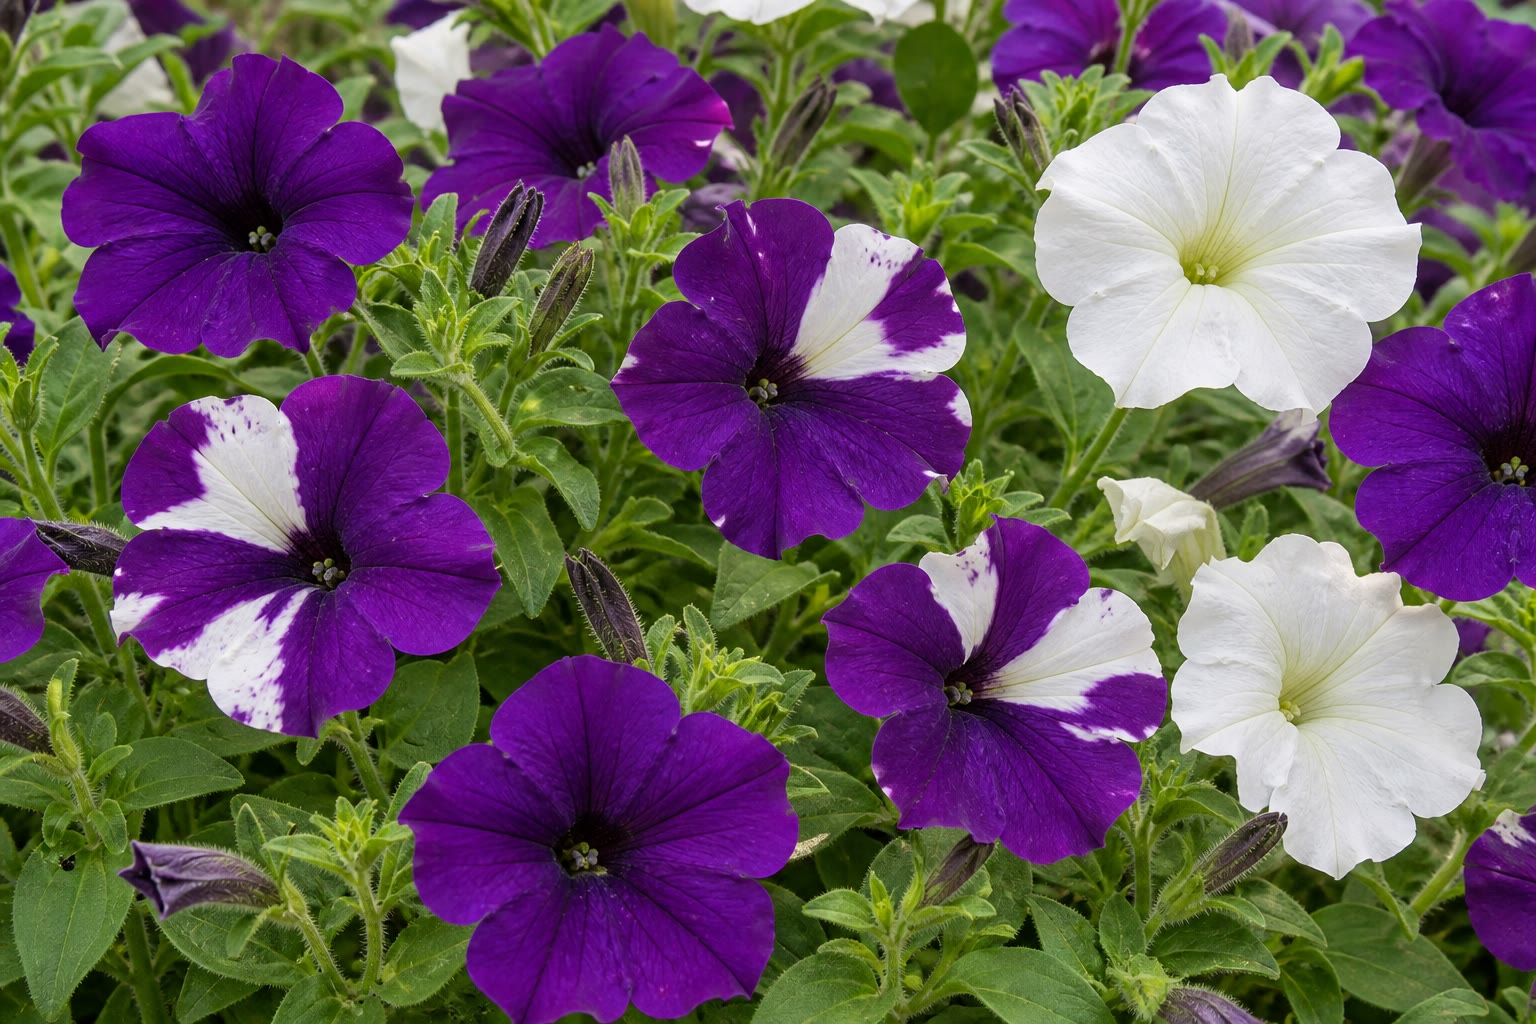
\includegraphics[width=0.46\linewidth]{images/book5/ai/b5-02-petunia-cosuppression.jpg}\hspace{0.04\linewidth}
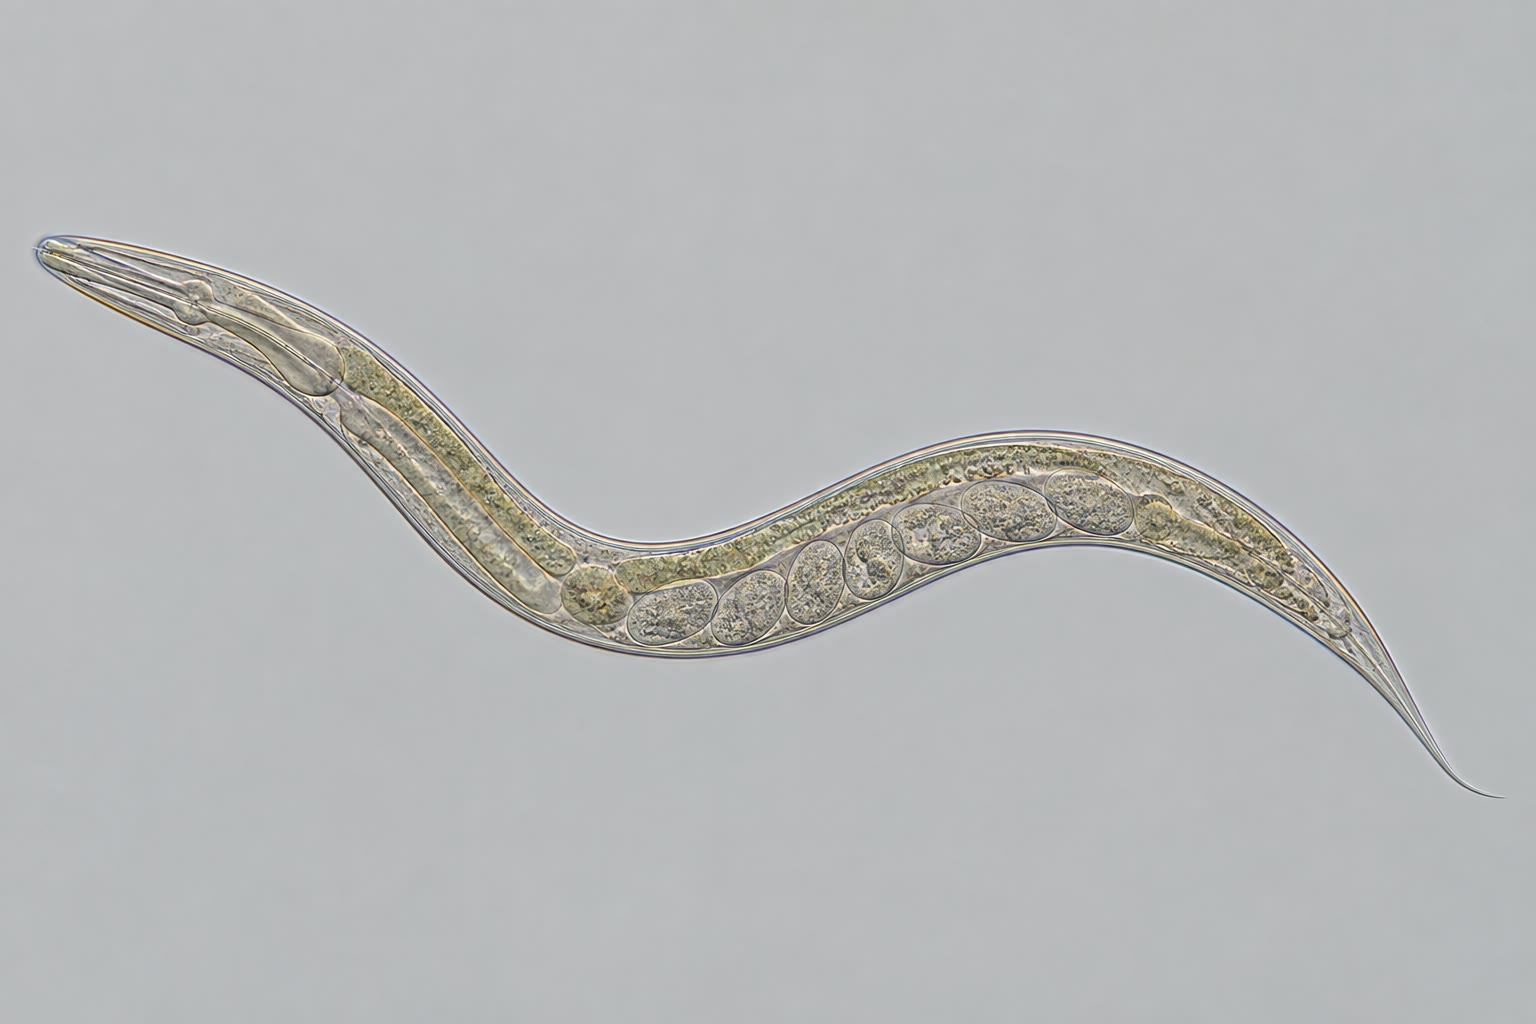
\includegraphics[width=0.46\linewidth]{images/book5/ai/b5-02-c-elegans.jpg}

{\small يسارًا: بتونيا تحمل مورّثة صباغ إضافية، وفيها القطاعات البيضاء
للكبت المشترك. يمينًا: الخيطية \emph{Caenorhabditis
elegans}، طولها نحو ميليمتر وهي شفافة، أسكت فيها RNA المزدوج المحقون
المورّثةَ المطابقة في الحيوان كله وفي ذريته.}
\end{omfigure}

\begin{definition}[RNA المكروية]\label{def:b3:rna-regulation:mirna}
\index{RNA مكروي!تخلّقه}\index{Drosha}\index{تسلسل البذرة}
\emph{\omterm{def:b3:rna-regulation:ncrna}{RNA المكروي}} مشفَّر في الجينوم --- في مورّثته الخاصة أو في إنترون
من مورّثة مشفِّرة للبروتين --- ويستنسخه بوليميراز RNA II نسخةً أولية
طويلة (pri-miRNA) تحوي دبوس شعر طوله نحو \qty{70}{nt}. وفي النواة
يقتطع \emph{Drosha}، وهو RNase III، الدبوسَ مع شريكه DGCR8 (فيصير
pre-miRNA)؛ ويحمله exportin-5 إلى الهيولى، حيث يزيل \omterm{def:b3:rna-regulation:rnai}{Dicer} العروة
فتبقى ثنائية طولها \qty{22}{nt}. ويُحمَّل أحد الطاقين في \omterm{def:b3:rna-regulation:rnai}{Argonaute}.
ويتعرف \omterm{def:b3:rna-regulation:ncrna}{RNA المكروي} الناضج أهدافه أساسًا عبر \emph{بذرته}، وهي
النوكليوتيدات 2 إلى 8، إذ تزاوج مواقع تقع عادةً في المنطقة غير
المترجمة 3$'$ من رسالة؛ أما بقية \omterm{def:b3:rna-regulation:ncrna}{RNA المكروي} فتزاوج مزاوجة ناقصة،
فلا يُقطع الهدف بل يُكبت: إذ يستدعي \omterm{def:b3:rna-regulation:rnai}{RISC} بروتينات تقصّر ذيل
poly(A) وتزيل القلنسوة وتثبط الترجمة، فتُحلَّل الرسالة أسرع. ولأن
البذرة سبعة نوكليوتيدات فقط، فللواحد من RNA المكروية مئات الأهداف، وأكثر
من نصف المورّثات البشرية المشفِّرة للبروتين تحمل مواقع محفوظة لواحد
على الأقل من عدة مئات من RNA المكروية البشرية المحققة.
\end{definition}

\begin{proof}[شواهد]
\emph{lin-4}، وهي مورّثة تلزم الدودة للانتقال من طورها اليرقي الأول
إلى الثاني، وجد لي وفاينباوم وأمبروس (1993) أنها لا تشفّر بروتينًا بل
RNA طوله \qty{22}{nt}، متممًا لسبعة مواقع في المنطقة غير المترجمة
3$'$ من رسالة \emph{lin-14}، وهي المورّثة التي كان معلومًا أنها
تكبتها. وحين تدخل اليرقة الطور الثاني يختفي بروتين LIN-14 مع بقاء
mRNA الخاص به: فالكبت إذن بعد الاستنساخ. ووجد راينهارت وزملاؤه (2000)
RNA ثانيًا من هذا القبيل هو \emph{let-7} يتحكم في الانتقالات اليرقية
اللاحقة؛ ووجدت باسكوينيلي (2000) \emph{let-7} في الذباب والبشر
بالتسلسل نفسه، فصارت طرفة دودية آليةً عامة.
\end{proof}

\begin{omfigure}
\begin{tikzpicture}[every node/.style={font=\scriptsize}, >=stealth]
  % nucleus box
  \draw[rounded corners=8pt, thick, gray!60, fill=gray!6] (-0.4,-1.1) rectangle (5.2,2.7);
  \node[gray, anchor=south west] at (-0.3,-1.05) {النواة};
  % gene and pri-miRNA
  \draw[very thick, omDef] (0,2.0) -- (2.4,2.0); \node[above] at (1.2,2.05) {مورّثة miRNA، بوليميراز II};
  \draw[->, thick] (1.2,1.85) -- (1.2,1.35);
  % hairpin
  \draw[thick, omThm!70!black] (0.2,1.0) -- (0.9,1.0) .. controls (1.0,1.0) and (1.05,0.9) .. (1.1,0.5) .. controls (1.15,0.1) and (1.25,0.1) .. (1.3,0.5) .. controls (1.35,0.9) and (1.4,1.0) .. (1.5,1.0) -- (2.2,1.0);
  \draw[thick, omThm!70!black] (1.1,0.5) -- (1.3,0.5);
  \node[below] at (1.2,0.0) {دبوس pri-miRNA};
  % Drosha
  \draw[thick, fill=omExo!35] (2.9,0.7) ellipse (0.55 and 0.28); \node at (2.9,0.7) {Drosha};
  \draw[->, thick] (2.3,0.85) -- (2.4,0.75);
  \draw[->, thick] (3.5,0.7) -- (4.2,0.7) node[midway, above] {قطع};
  % pre-miRNA
  \draw[thick, omThm!70!black] (4.3,0.9) .. controls (4.5,0.9) and (4.55,0.4) .. (4.6,0.1) .. controls (4.65,-0.2) and (4.75,-0.2) .. (4.8,0.1) .. controls (4.85,0.4) and (4.9,0.9) .. (5.1,0.9);
  \node[below, align=center] at (4.7,-0.25) {pre-miRNA\\\qty{70}{nt}};
  % export
  \draw[->, thick] (5.35,0.4) -- (6.3,0.4) node[midway, above, xshift=0.2cm] {exportin-5};
  % cytoplasm
  \node[gray, anchor=north west] at (5.5,2.65) {الهيولى};
  \draw[thick, fill=omExo!35] (6.9,0.4) ellipse (0.5 and 0.28); \node at (6.9,0.4) {Dicer};
  \draw[->, thick] (7.45,0.4) -- (8.1,0.4);
  \draw[thick, omThm!70!black] (8.2,0.55) -- (9.6,0.55); \draw[thick, omThm!70!black] (8.35,0.25) -- (9.75,0.25);
  \node[below, align=center] at (8.95,0.15) {ثنائية \qty{22}{nt}};
  \draw[->, thick] (8.95,-0.4) -- (8.95,-0.9) node[midway, right] {يُحمَّل طاق واحد};
  % RISC on mRNA
  \draw[thick, fill=omProp!35] (8.95,-1.45) ellipse (0.85 and 0.35); \node at (8.95,-1.45) {Argonaute};
  \draw[thick, omThm!70!black] (8.3,-1.85) -- (9.6,-1.85);
  \draw[very thick, omDef] (5.6,-2.15) -- (11.4,-2.15);
  \node[below] at (6.4,-2.2) {mRNA: المنطقة المشفِّرة}; \node[below] at (10.3,-2.2) {UTR 3$'$، موقع الهدف};
  \draw[omDef, thick] (11.4,-2.15) -- (11.8,-2.15) node[right] {AAAA};
  \draw[->, thick, omThm] (9.9,-1.5) -- (10.9,-1.5) node[right, align=left] {نزع الأدنين،\\تحلل، ترجمة\\أقل};
  \node[below, align=center] at (8.95,-2.7) {البذرة (النوكليوتيدات 2--8)\\تزاوج الموقع};
\end{tikzpicture}

{\small تخلّق \omterm{def:b3:rna-regulation:ncrna}{RNA مكروي}. يقتطع \omterm{def:b3:rna-regulation:mirna}{Drosha} الدبوسَ من النسخة الأولية في
النواة، ثم يُصدَّر، ويقلّمه \omterm{def:b3:rna-regulation:rnai}{Dicer} إلى ثنائية طولها \qty{22}{nt}،
ويُحمَّل أحد الطاقين في \omterm{def:b3:rna-regulation:rnai}{Argonaute}. وتزاوج البذرةُ موقعًا في المنطقة
غير المترجمة 3$'$ من رسالة، فيُنزع أدنينها وتُحلَّل وتُترجم أقل.}
\end{omfigure}

\begin{theorem}[ما يفعله RNA مكروي بمستوى رسالة وبسرعتها]\label{thm:b3:rna-regulation:mirna-kinetics}
\index{عمر نصف mRNA}\index{زمن الاستجابة}
تُصنع الرسالة بمعدل ثابت $k$ وتُحلَّل بمعدل من الرتبة الأولى $\gamma$؛
ويضيف \omterm{def:b3:rna-regulation:ncrna}{RNA مكروي} حاضر بمستوى $R$ حدَّ تحلل $\gamma' R\, m$. عندئذٍ
يخضع مستوى mRNA، أي $m(t)$، للعلاقة
\[
\frac{\mathrm{d}m}{\mathrm{d}t} = k - (\gamma + \gamma' R)\, m,
\qquad
m^{*} = \frac{k}{\gamma + \gamma' R},
\qquad
m(t) = m^{*} + (m_{0} - m^{*})\,e^{-(\gamma + \gamma' R)t}.
\]
يخفض \omterm{def:b3:rna-regulation:ncrna}{RNA المكروي} الحالة المستقرة بالعامل $1 + \gamma' R/
\gamma$ ويقصّر ثابت الزمن لكل تغير في $m$ من $1/\gamma$ إلى
$1/(\gamma + \gamma' R)$ بالعامل نفسه. فالمورّثة الخاضعة لتنظيم \omterm{def:b3:rna-regulation:ncrna}{RNA مكروي}
أهدأ وأسرع معًا: إذ تبلغ حالة مستقرة جديدة أبكر بعد تغير مروّجها،
وتُخمَد التقلبات في استنساخها.
\end{theorem}
\begin{proof}
المعادلة خطية بمعاملات ثابتة؛ ونقطتها الثابتة $m^{*}$ حيث ينعدم الطرف
الأيمن، وبوضع $u = m - m^{*}$ نحصل على
$\mathrm{d}u/\mathrm{d}t = -(\gamma + \gamma' R)\,u$، ومنه الأسّي.
وزمن نصف الاقتراب هو $\ln 2/(\gamma + \gamma'
R)$، و$\gamma = \ln 2 / t_{1/2}$ حيث $t_{1/2}$ عمر النصف الطبيعي
للرسالة.
\end{proof}

\begin{example}[كبت بأربعة أمثال]\label{ex:b3:rna-regulation:fourfold}
رسالة عمر نصفها الطبيعي \qty{30}{min} ($\gamma =
\qty{0.023}{min^{-1}}$)، تُستنسخ بمعدل $k = 2$ جزيء في الدقيقة، تستقر
عند $m^{*} = 2/0.023 \approx 87$ نسخة في الخلية وتحتاج
\qty{30}{min} لتقطع نصف الطريق إلى مستوى جديد بعد تغير مروّجها. \omterm{def:b3:rna-regulation:ncrna}{وRNA
مكروي} يثلّث معدل تحللها ($\gamma' R = 3\gamma$) ينزل بها إلى $22$
نسخة ويقصّر زمن النصف إلى \qty{7.5}{min}. والأرقام نفسها، مقروءةً
عكسًا، تبين لماذا يكون للأنماط المحذوفة من miRNA أنماط ظاهرية خفيفة
غالبًا: فتغير بأربعة أمثال في رسالة هي نفسها مُهدّأة في مراحل تالية
قد يترك الكائن سويًا تقريبًا، ويظهر الأثر تحت الإجهاد أو في التوقيت.
\end{example}

\begin{omfigure}
\begin{tikzpicture}
\begin{axis}[
  width=0.7\linewidth, height=5.6cm,
  axis x line=bottom, axis y line=left,
  xmin=0, xmax=120, ymin=0, ymax=100,
  xlabel={الزمن بعد فتح المروّج (دقيقة)}, ylabel={mRNA في الخلية},
  xlabel style={font=\small, at={(axis description cs:0.5,-0.12)}, anchor=north},
  ylabel style={font=\small},
  tick label style={font=\small}, xtick={0,30,60,90,120}, ytick={0,22,50,87},
  clip=false,
]
\addplot[very thick, omDef, domain=0:120, samples=80] {87*(1-exp(-0.0231*x))};
\addplot[very thick, omThm, domain=0:120, samples=80] {21.7*(1-exp(-0.0924*x))};
\addplot[dashed, gray, domain=0:120, samples=2] {87};
\addplot[dashed, gray, domain=0:120, samples=2] {21.7};
\node[font=\scriptsize, omDef, anchor=south west] at (axis cs:5,90) {بلا RNA مكروي: $m^{*} = 87$، زمن النصف \qty{30}{min}};
\node[font=\scriptsize, omThm, anchor=south west] at (axis cs:40,24) {مع RNA مكروي، $\gamma' R = 3\gamma$: $m^{*} = 22$، زمن النصف \qty{7.5}{min}};
\end{axis}
\end{tikzpicture}

{\small ارتفاع رسالة بعد فتح مروّجها، بأرقام
\cref{ex:b3:rna-regulation:fourfold}. يخفض \omterm{def:b3:rna-regulation:ncrna}{RNA المكروي} المستوى
المستقر أربعة أمثال ويبلغه في ربع الزمن.}
\end{omfigure}

\begin{method}[خفض مورّثة بالتداخل الرنائي]\label{met:b3:rna-regulation:knockdown}
\index{خفض التعبير}\index{shRNA}
لإسكات مورّثة دون مساس بجزيء DNA الخاص بها: (1) اختر تسلسلًا طوله
\qty{21}{nt} يخص رسالتها وحدها، متجنبًا تطابق البذرة مع مورّثات أخرى؛
(2) أوصله ثنائيةَ \omterm{def:b3:rna-regulation:ncrna}{siRNA} مركّبة (عابرة، بضعة أيام) أو RNA قصيرًا على
شكل دبوس (shRNA) يُعبَّر عنه من ناقل، فيعالجه \omterm{def:b3:rna-regulation:rnai}{Dicer} باستمرار؛ وفي
الديدان أطعم الحيوانات بكتيريا تعبّر عن RNA المزدوج؛ (3) قِس الرسالة
بتفاعل PCR الكمي والبروتين بالتلطيخ المناعي، متوقعًا فقدًا بنسبة
\qtyrange{70}{95}{\%} لا غيابًا تامًا كما في الحذف؛ (4) اضبط الآثار
خارج الهدف بجزيء \omterm{def:b3:rna-regulation:ncrna}{siRNA} ثانٍ غير متداخل وبإنقاذ بنسخة من المورّثة مقاومة
\omterm{def:b3:rna-regulation:rnai}{للتداخل الرنائي}. فالخفض فقدُ وظيفة جزئي وعكوس؛ والعلاجات الجينية
المعتمدة اليوم على هذا المبدأ توصل \omterm{def:b3:rna-regulation:ncrna}{siRNA} ضد رسائل كبدية
(ترانسثيريتين، PCSK9) مقرونة بسكر يلتقطه الخلية الكبدية.
\end{method}

\section{RNA صغيرة تحرس الجينوم}

\begin{definition}[piRNA وإسكات العناصر القافزة]\label{def:b3:rna-regulation:pirna}
\index{piRNA!البنغ بونغ}\index{إسكات العناصر القافزة}\index{خلل التخلّق الهجين}
\emph{\omterm{def:b3:rna-regulation:ncrna}{piRNA}} جزيئات RNA طولها \numrange{26}{31} نوكليوتيدًا، تُصنع بلا
\omterm{def:b3:rna-regulation:rnai}{Dicer} من نسخ طويلة مفردة الطاق من \emph{عناقيد \omterm{def:b3:rna-regulation:ncrna}{piRNA}} الجينومية
--- وهي مقابر لنسخ معطوبة من عناصر قافزة --- وتُحمَّل في أسرة PIWI
الفرعية من بروتينات \omterm{def:b3:rna-regulation:rnai}{Argonaute} في السلالة الجنسية. \omterm{def:b3:rna-regulation:ncrna}{وpiRNA} المضاد لعنصر
قافز يوجّه قطع نسخ ذلك العنصر؛ ويصير الجزء المقطوع \omterm{def:b3:rna-regulation:ncrna}{piRNA} جديدًا ذا
معنى، يقطع بدوره نسخ العناقيد ليصنع مزيدًا من \omterm{def:b3:rna-regulation:ncrna}{piRNA} المضادة --- وهي
دورة \emph{البنغ بونغ}، وهي تضخيم يستهدف أي عنصر قافز نشط في حينه.
كما توجّه بروتينات PIWI النووية مثيلة H3K9 \omterm{def:b3:chromatin-epigenetics:methylation}{ومثيلة DNA} على النسخ
الجينومية للعنصر، فتصل RNA بعلامات \omterm{def:b3:chromatin-epigenetics:nucleosome}{الصبغين} في
\cref{ch:b3:chromatin-epigenetics}. وتودع الأم \omterm{def:b3:rna-regulation:ncrna}{piRNA} في البيضة؛
فالأنثى التي لم تلق سلالتها عنصرًا قافزًا قط لا \omterm{def:b3:rna-regulation:ncrna}{piRNA} عندها ضده،
وذريتها من ذكر يحمله عقيمة --- وهو
\emph{خلل التخلّق الهجين}، رئي أول ما رئي في تهجينات \emph{Drosophila}
بين سلالات مخبرية وأخرى برية.
\end{definition}

\begin{proposition}[إسكات الصبغين بتوجيه RNA]\label{prop:b3:rna-regulation:rddm}
\index{مثيلة DNA بتوجيه RNA}
في النبات مسلك مخصص --- يستنسخ بوليميراز RNA IV موضعًا، ويجعله
بوليميراز RNA معتمد على RNA مزدوجًا، ويقطع \omterm{def:b3:rna-regulation:rnai}{Dicer} منه \omterm{def:b3:rna-regulation:ncrna}{siRNA} بطول
\qty{24}{nt}، ويحملها \omterm{def:b3:rna-regulation:rnai}{Argonaute}~4 عائدةً إلى النسخ الوليدة لبوليميراز
V عند الموضع نفسه ويستدعي ناقلة الميثيل DRM2 --- فيمثيل DNA العناصر
القافزة والمتتاليات المكررة؛ وهو آلية \omterm{prop:b3:chromatin-epigenetics:examples}{الطفرة الجانبية}. وفي خميرة
الانشطار تستدعي \omterm{def:b3:rna-regulation:ncrna}{siRNA} الآتية من التكرارات المركزية ناقلةَ ميثيل H3K9
فتبني \omterm{def:b3:chromatin-epigenetics:nucleosome}{الصبغين المتغاير} الذي يحتاجه القسيم المركزي. وفي الحالتين يجد
RNA موضعًا في الجينوم بالتتام فتُكتب هناك علامة صبغينية: نوعية
التسلسل، ذاتية التعزيز، وقابلة للتوريث عبر الانقسامات.
\end{proposition}

\section{حياة رسالة}

\begin{definition}[التشذيب المنظَّم]\label{def:b3:rna-regulation:splicing}
\index{تشذيب بديل!تنظيمه}\index{بروتين SR}\index{hnRNP}\index{تخطي الإكسون}
يُنتج التشذيب البديل رسائل مختلفة من مورّثة واحدة عبر \emph{تخطي
الإكسون}، أو بالاختيار بين إكسونين متنافيين، أو بإبقاء إنترون، أو
باستعمال مواقع تشذيب بديلة عند 5$'$ أو 3$'$. وتنظمه بروتينات رابطة
لجزيء RNA ترتبط بعناصر تسلسلية في الإكسونات والإنترونات قرب موقع تشذيب:
فإن \emph{بروتينات SR} المرتبطة بمعزِّزات إكسونية تستدعي الجسيم المشذِّب
وتعزز إدراج الإكسون، وبروتينات \emph{hnRNP} المرتبطة بمُسكتات تمنعه،
وتحدد النسبة بين الصنفين النتيجةَ في خلية بعينها. وأكثر من
\qty{90}{\%} من المورّثات البشرية متعددة الإكسونات تُشذَّب تشذيبًا
بديلًا؛ ومورّثة \emph{Dscam} في \emph{Drosophila}، بأربع كتل من
الإكسونات المتنافية (12 و48 و33 و2 بدائل)، تستطيع إنتاج \num{38016}
بروتين مختلف، يعبّر كل عصبون عن طقم مختلف يتيح لتفرعاته أن يتعرف
بعضها بعضًا فيتجنبه.
\end{definition}

\begin{proof}[شواهد]
يقرر جنسَ ذبابة الفاكهة شلالٌ من التشذيب. ففي الإناث تصنع مورّثة
\emph{Sex-lethal} (\emph{Sxl}) بروتينًا فاعلًا؛ وSXL بروتين رابط
لجزيء RNA يحجب موقع تشذيب في نسخته هو
(فيُتخطى إكسون يحمل رامزة وقف ويستمر صنع البروتين)
ويحجب موقعًا في نسخة \emph{transformer}، ففارضًا التشذيب
الأنثوي؛ ثم يرتبط TRA مع TRA-2 بمعزِّز إكسوني في نسخة
\emph{doublesex} فيوجّه الصورة الأنثوية من عامل الاستنساخ DSX. وفي
الذكور، حيث لا SXL، تأخذ كل نسخة من هذه النسخ التشذيبَ الافتراضي،
فتحوي \emph{transformer} رامزة وقف، ويخرج DSX في صورته الذكرية. وكل
صفة جنسية متغايرة في الذبابة تتبع أيَّ DSX صُنع؛ والأنثى التي طُفرت
فيها \emph{tra} تتطور ذكرًا.
\end{proof}

\begin{definition}[ثبات الرسالة وتوطينها]\label{def:b3:rna-regulation:stability}
\index{عنصر غني بالأدنين واليوراسيل}\index{توطين mRNA}\index{عنصر مستجيب للحديد}
يتراوح \emph{عمر نصف} الرسالة بين دقائق وأيام، وتحدده عناصر في منطقتها
غير المترجمة 3$'$. فإن \emph{العناصر الغنية بالأدنين واليوراسيل}
(تكرارات AUUUA) في رسائل السيتوكينات وعوامل النمو والمورّثات الورمية
الأولية ترتبط بها بروتينات تستدعي نازعات الأدنين فتعطي أعمار نصف
\qtyrange{10}{30}{min}، حتى تُنتج دفقةُ الاستنساخ دفقةَ بروتين لا
أكثر؛ والطفرات التي تزيلها تسبب فرط التعبير، وتسبب السرطان في بعض
المورّثات الورمية الأولية. و\emph{عناصر التوطين}، وهي مبنية غالبًا،
ترتبط بها وسائط تصل الرسالة بمحرّك: فرسالتا \emph{bicoid}
و\emph{oskar} تُحملان إلى قطبي بيضة الذبابة بالداينين
والكينيزين على الأنيبيبات الدقيقة، ورسالة الأكتين $\beta$ إلى الحافة
الأمامية في الخلية الليفية، ورسائل البروتينات المشبكية إلى التغصنات
حيث تُترجم عند الطلب. أما \emph{العنصر المستجيب للحديد}
(IRE)، وهو ساق وعروة يرتبط بها البروتينان المنظمان للحديد IRP1 و
IRP2 عند شحّ الحديد، فيؤدي وظيفتين متعاكستين من موضعين: ففي المنطقة
غير المترجمة 5$'$ من رسالة الفيريتين يحجب IRP المرتبط الريبوزومَ؛ وفي
المنطقة غير المترجمة 3$'$ من رسالة مستقبل الترانسفيرين يحمي IRP
المرتبط النسخةَ من نوكلياز.
\end{definition}

\begin{example}[الحديد، مقروءًا بدبوس واحد]\label{ex:b3:rna-regulation:iron}
حين يقلّ الحديد يرتبط IRP بالرسالتين معًا: فلا يُترجم الفيريتين، وهو
بروتين الخزن، ويثبت مستقبل الترانسفيرين الذي يستورد الحديد فيكثر ---
فتخزن الخلية أقل وتستورد أكثر. وحين يكثر الحديد يحوّل IRP1 إلى
أكونيتاز (إذ يكتسب عنقود حديد وكبريت ويفقد ألفته لجزيء RNA) ويطلق تحلل
IRP2: فيُترجم الفيريتين، وتتحلل رسالة المستقبل في دقائق، فتخزن الخلية
أكثر وتستورد أقل. ولا حاجة إلى تغير في الاستنساخ. والطفرة النقطية في
IRE الفيريتين التي تمنع ارتباط IRP تسبب تركيبًا بنيويًا للفيريتين
ومتلازمة فرط الفيريتين الوراثي مع الساد.
\end{example}

\begin{omfigure}
\begin{tikzpicture}[every node/.style={font=\scriptsize}, >=stealth]
  \foreach \yy/\state in {2.2/{حديد قليل}, -0.9/{حديد كثير}} {
    \node[left, font=\small\bfseries] at (-0.2,\yy+0.35) {\state};
    % ferritin mRNA
    \draw[very thick, omDef] (0.3,\yy+0.6) -- (4.6,\yy+0.6); \node[below] at (3.3,\yy+0.4) {رسالة الفيريتين};
    \draw[thick, omThm!70!black] (0.9,\yy+0.6) .. controls (0.9,\yy+1.15) and (1.3,\yy+1.15) .. (1.3,\yy+0.6); \node[below] at (1.1,\yy+0.55) {IRE};
    \draw[fill=omDef!20, thick] (2.2,\yy+0.42) rectangle (4.4,\yy+0.78);
    % TfR mRNA
    \draw[very thick, omDef] (6.2,\yy+0.6) -- (10.6,\yy+0.6); \node[below, font=\tiny] at (7.1,\yy+0.4) {رسالة مستقبل الترانسفيرين};
    \draw[fill=omDef!20, thick] (6.4,\yy+0.42) rectangle (8.6,\yy+0.78);
    \foreach \x in {9.0,9.5,10.0} \draw[thick, omThm!70!black] (\x,\yy+0.6) .. controls (\x,\yy+1.1) and (\x+0.35,\yy+1.1) .. (\x+0.35,\yy+0.6);
    \node[below, font=\tiny] at (9.9,\yy+0.55) {عناصر IRE (UTR 3$'$)};
  }
  % low iron: IRP bound
  \draw[thick, fill=omProp!40] (1.1,3.35) ellipse (0.4 and 0.24); \node at (1.1,3.35) {IRP};
  \node[right, omThm] at (1.55,3.35) {الريبوزوم محجوب: لا فيريتين};
  \foreach \x in {9.18,9.68,10.18} { \draw[thick, fill=omProp!40] (\x,3.35) ellipse (0.28 and 0.2); }
  \node[above, omMeth!70!black] at (9.7,3.75) {محمية من النوكلياز: مستقبل ثابت وفير};
  \node[below, omMeth!70!black] at (1.1,1.75) {تخزن أقل};
  \node[below, omMeth!70!black] at (7.4,1.75) {تستورد أكثر};
  % high iron: IRP off
  \node[right, omMeth!70!black] at (1.55,0.25) {مترجمة: يُصنع الفيريتين};
  \node[right, omThm, align=left] at (10.7,-0.3) {نوكلياز:\\تتحلل mRNA};
  \node[below, omThm] at (1.1,-1.35) {تخزن أكثر};
  \node[below, omThm] at (7.4,-1.35) {تستورد أقل};
\end{tikzpicture}

{\small \omterm{def:b3:rna-regulation:stability}{العنصر المستجيب للحديد}. عند قلة الحديد يرتبط البروتين المنظم
للحديد بدبابيس IRE: فيحجب الترجمة عند النهاية 5$'$ من رسالة
الفيريتين، ويحجب نوكليازًا عند النهاية 3$'$ من رسالة مستقبل
الترانسفيرين. وعند كثرة الحديد يطلق البروتين كليهما: فيُصنع
الفيريتين، وتتحلل رسالة المستقبل.}
\end{omfigure}

\begin{proposition}[التحكم في الترجمة]\label{prop:b3:rna-regulation:translation}
\index{تحكم في الترجمة}\index{eIF2}\index{مفتاح ريبوزي}\index{إطار قراءة مفتوح أعلى}
خطوة البدء هي نقطة التحكم المعتادة في الترجمة. فَفَسْفَرةُ عامل البدء
\emph{eIF2} بكينازات تستشعر الجوع إلى الأحماض الأمينية، أو البروتينات
غير المنطوية، أو RNA الفيروسي المزدوج، أو نقص الهيم، توقف البدء العام
في دقائق، مع استثناء رسائل قليلة ذات سمات خاصة --- وأبرزها ذوات
\emph{أطر القراءة المفتوحة الأعلى}، وهي أطر قصيرة في المنطقة غير
المترجمة 5$'$ تحبس الريبوزومات عادةً وتُتخطى تحت
الإجهاد، فتُصنع عوامل الاستجابة للإجهاد (GCN4 في الخميرة وATF4 في
الثدييات) في اللحظة التي لا يُصنع فيها كل ما عداها. أما عامل ربط
القلنسوة eIF4E فتبقيه بروتينات رابطة للعامل 4E خاملًا حتى تفسفرها كيناز
إشارات النمو mTOR: فلا تترجم الخلية بكامل معدلها إلا حين تأذن
المغذيات وعوامل النمو. وفي البكتيريا تفعل \emph{المفاتيح الريبوزية}
ذلك بلا بروتين: إذ ترتبط منطقة 5$'$ مبنية بمستقلَب (ثنائي فوسفات
الثيامين، أو S-أدينوزيل الميثيونين، أو بورين) فتعيد الانطواء عند
الارتباط لتدفن موقع ربط الريبوزوم أو لتكوّن منهيًا للاستنساخ، فتُغلق
سبيلة اصطناعية حين يكثر ناتجها.
\end{proposition}

\begin{omfigure}
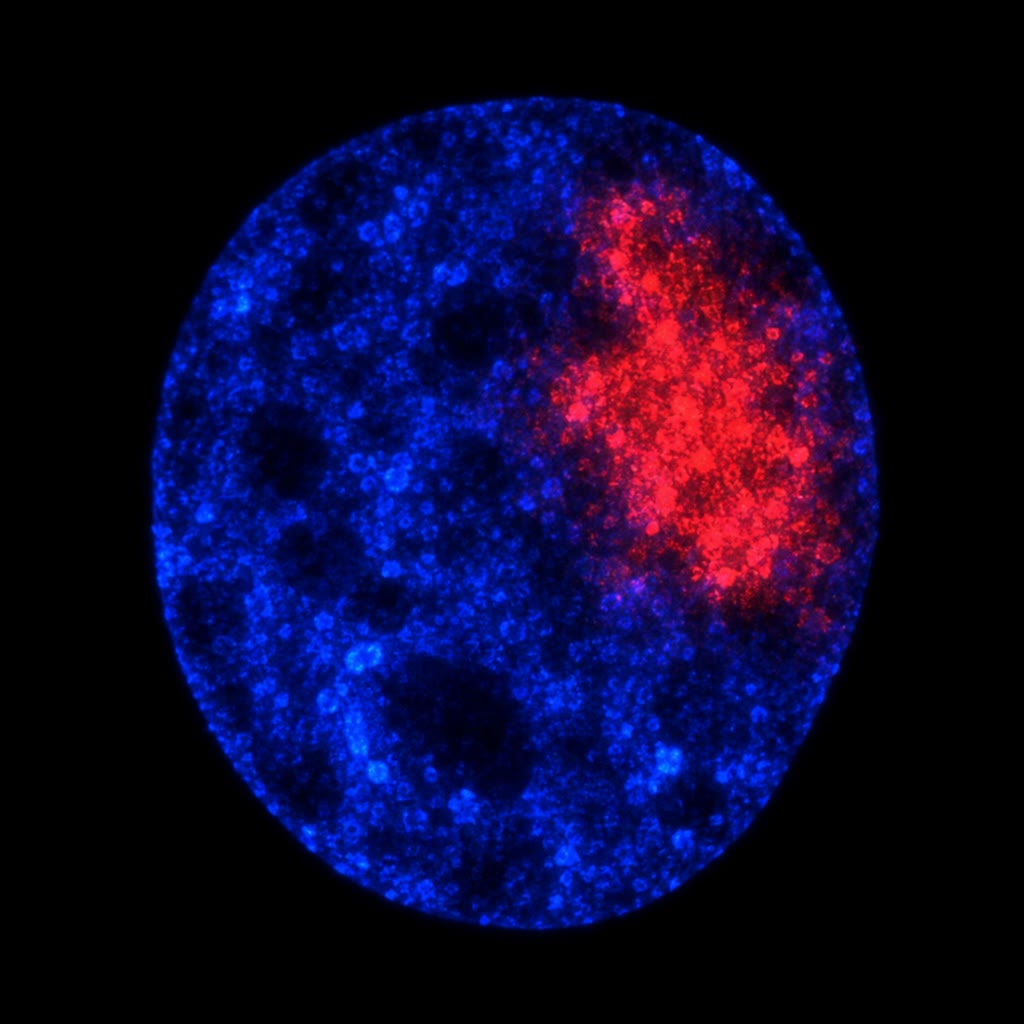
\includegraphics[width=0.36\linewidth]{images/book5/ai/b5-02-lncrna-nucleus.jpg}

{\small \omterm{def:b3:rna-regulation:ncrna}{RNA طويل غير مشفِّر} في العمل: نسخة \emph{\omterm{def:b3:chromatin-epigenetics:x-inactivation}{Xist}}
(بالأحمر)، مكشوفة بالتهجين المتألق، تغلّف إقليم أحد
صبغيي X في نواة أنثوية (وDNA بالأزرق).}
\end{omfigure}

\begin{remark}[ما يشتريه التحكم بعد الاستنساخ]\label{rem:b3:rna-regulation:why}
يعمل التحكم الاستنساخي عبر النواة، بتأخر دقائق إلى ساعات قبل أن
تُصنع رسالة جديدة وتُصدَّر وتُترجم. أما التحكم في الرسالة نفسها
فيعمل حيث يُحتاج إلى البروتين، في ثوانٍ إلى دقائق، ويمكن أن يكون
موضعيًا: تغصن واحد يترجم رسالة واحدة عند مشبك واحد، وحافة أمامية
لخلية ليفية تصنع الأكتين حيث تزحف. وهو يجعل من مورّثة واحدة بروتينات
كثيرة، ويتيح لإشارة واحدة --- حديد، أو حمض أميني، أو \omterm{def:b3:rna-regulation:ncrna}{RNA مكروي} ---
أن تنسّق مئات الرسائل دفعةً واحدة دون مساس بأي مروّج.
\end{remark}

\section{تمارين}

\begin{exercise}[$\star$]\label{exo:b3:rna-regulation:1}
ميّز بين miRNA \omterm{def:b3:rna-regulation:ncrna}{وsiRNA} \omterm{def:b3:rna-regulation:ncrna}{وpiRNA} من حيث المنشأ والطول والاعتماد على \omterm{def:b3:rna-regulation:rnai}{Dicer}
وما تفعله بأهدافها.
\end{exercise}

\begin{exercise}[$\star$]\label{exo:b3:rna-regulation:2}
تتبّع تخلّق \omterm{def:b3:rna-regulation:ncrna}{RNA مكروي} من مورّثته إلى رسالة مكبوتة، مسمّيًا الإنزيم
عند كل قطع.
\end{exercise}

\begin{exercise}[$\star$]\label{exo:b3:rna-regulation:3}
لماذا أسكت حقنُ RNA ذي المعنى من \emph{unc-22} في الديدان المورّثةَ
في التجارب الأولى، وما الذي غيّره فاير وميلو؟
\end{exercise}

\begin{exercise}[$\star$]\label{exo:b3:rna-regulation:4}
ماذا يحدث للفيريتين ولمستقبل الترانسفيرين حين تُجوَّع الخلية من
الحديد؟ وأي خطوة من خطوات التعبير هي المتحكَّم فيها في كل من
الحالتين؟
\end{exercise}

\begin{exercise}[$\star\star$]\label{exo:b3:rna-regulation:5}
رسالة عمر نصفها \qty{2}{h} وتُصنع بمعدل $5$ جزيئات في الدقيقة. احسب
مستواها المستقر، ثم المستوى وزمن النصف حين يضاعف \omterm{def:b3:rna-regulation:ncrna}{RNA مكروي} معدل
تحللها.
\end{exercise}

\begin{exercise}[$\star\star$]\label{exo:b3:rna-regulation:6}
تطابق بذرةٌ من سبعة نوكليوتيدات تسلسلًا عشوائيًا باحتمال $4^{-7}$.
في مجموعة من \num{20000} رسالة مناطقُها غير المترجمة 3$'$ بمتوسط
\qty{1000}{nt}، كم موقعًا تطابق بذرةُ \omterm{def:b3:rna-regulation:ncrna}{RNA مكروي} واحد مصادفةً؟ وما
الذي يميز الهدف الحقيقي إذن؟
\end{exercise}

\begin{exercise}[$\star\star$]\label{exo:b3:rna-regulation:7}
تنبأ بجنس ذبابة (أ) فيها طفرة فقدِ وظيفة في \emph{tra} وصبغيا X؛
(ب) تعبّر عن TRA من مورث نقيل بنيوي، ولها صبغي X واحد؛ (ج) تخلو من
\emph{dsx} كليًا.
\end{exercise}

\begin{exercise}[$\star\star$]\label{exo:b3:rna-regulation:8}
رسالة مورّثة ورمية أولية عمر نصفها عادةً \qty{15}{min} بسبب \omterm{def:b3:rna-regulation:stability}{عنصر غني
بالأدنين واليوراسيل}. وأزال انتقالٌ صبغي العنصرَ فصار عمر النصف \qty{3}{h}. بأي عامل
يرتفع مستوى البروتين إذا لم تتغير الترجمة ولا تحلل البروتين؟ ولماذا
يكون هذا مسرطنًا مع أن البروتين سوي؟
\end{exercise}

\begin{exercise}[$\star\star$]\label{exo:b3:rna-regulation:9}
سلالة مخبرية من \emph{Drosophila} تخلو من عناصر P؛ وسلالة برية
تحملها. تنبأ بخصوبة ذرية (أ) إناث مخبرية $\times$ ذكور برية،
(ب) إناث برية $\times$ ذكور مخبرية، وفسّر عدم التناظر \omterm{def:b3:rna-regulation:pirna}{بجزيئات piRNA}.
\end{exercise}

\begin{exercise}[$\star\star\star$]\label{exo:b3:rna-regulation:10}
باستعمال \cref{thm:b3:rna-regulation:mirna-kinetics}، برهن على أن
البروتين المصنوع من رسالة يتقلب أقل، نسبيًا، حين تكون الرسالة خاضعة
لتنظيم \omterm{def:b3:rna-regulation:ncrna}{RNA مكروي}، عند تساوي متوسط مستوى الرسالة. (فالبروتين يتوسط الرسالة
على مدى عمره هو، والرسالة تتجدد أسرع.) ولماذا قد تدفع الخلية ثمن
\omterm{def:b3:rna-regulation:ncrna}{RNA مكروي} ومعدل استنساخ أعلى لتبلغ المتوسط نفسه؟
\end{exercise}

\begin{exercise}[$\star\star\star$]\label{exo:b3:rna-regulation:11}
في الديدان يصنع بوليميراز RNA معتمد على RNA جزيئاتِ \omterm{def:b3:rna-regulation:ncrna}{siRNA} ثانوية من
رسالة الهدف؛ ولا وجود له في الثدييات. تنبأ، في كل من الحالتين، هل
يدوم الإسكات بحقنة واحدة من RNA مزدوج عبر انقسامات خلوية كثيرة وهل
ينتشر إلى أنسجة أخرى، وفسّر النتيجة الطبية على أدوية \omterm{def:b3:rna-regulation:ncrna}{siRNA}.
\end{exercise}

\begin{exercise}[$\star\star\star$]\label{exo:b3:rna-regulation:12}
lncRNA موصوف حديثًا يُعبَّر عنه في القلب. صمّم التجارب التي تميز بين
(أ) RNA وظيفي، و(ب) فعل استنساخ وظيفي لا شأن لجزيء RNA الناتج عنه،
و(ج) ضجيج، وقل ما الذي تتنبأ به كل حالة من نتيجة.
\end{exercise}

\section{مسألة: مؤقّت دودة}

\begin{problem}[{مسألة نهاية الأسبوع --- مفتاح \emph{lin-4}/\emph{lin-14}
في الدودة موقوتًا بحركية الرسالة، وRNA محقون يُمدَّد عبر انقسامات
جنين ويُنقذ بالتضخيم، وحُصَين الحديد مقيسًا، وعدّ للتشذيب،
وتنتهي إلى مقدار الكبت وزمن نصف المفتاح وعدد الانقسامات التي تنجو
فيها إشارة غير مضخَّمة}]
\label{pb:b3:rna-regulation:1}
معطيات: رسالة \emph{lin-14} تُصنع بمعدل $k = 3$ جزيئات في الدقيقة
في الخلية وعمر نصفها \qty{40}{min}. وبروتين LIN-14 يُصنع بمعدل
$\beta = 2$ لكل رسالة في الدقيقة وعمر نصفه \qty{3}{h}. ومن بداية
الطور اليرقي الثاني يتراكم RNA الخاص بالمورّثة \emph{lin-4} فيضيف حدَّ تحلل
$\gamma' R = 3\gamma$ إلى الرسالة، ويُنصّف $\beta$ بحجبه البدء.
ويتطور جنين الدودة من خلية واحدة إلى نحو \num{550} خلية عند الفقس؛
وللبالغ \num{959} خلية جسدية.

\medskip
\noindent\textbf{الجزء الأول --- الرسالة.}
\begin{enumerate}
  \item احسب $\gamma$ ومستوى رسالة \emph{lin-14} المستقر قبل ظهور
        \emph{lin-4}.
  \item احسب معدل تحلل البروتين ومستوى بروتين LIN-14 المستقر.
  \item متى حضر \emph{lin-4}، احسب مستوى الرسالة الجديد وثابت الزمن
        الجديد للرسالة.
  \item احسب الحالة المستقرة الجديدة للبروتين، ومقدار الكبت الكلي
        على البروتين.
  \item بعد كم من الزمن من ظهور \emph{lin-4} تبلغ الرسالة نصف الطريق
        إلى مستواها الجديد؟ وكم للبروتين --- وأي خطوة تحدّ سرعة
        المفتاح؟
  \item وجدت التجارب الأولى البروتين قد زال والرسالة ما تزال مكشوفة.
        أيوافق ذلك أرقامك؟ وما نسبة الباقي من الرسالة؟
\end{enumerate}

\medskip
\noindent\textbf{الجزء الثاني --- التمديد والتضخيم.}
\begin{enumerate}[resume]
  \item يُحقن مبيض دودة بمقدار $10^{6}$ جزيء من RNA المزدوج، تُقتسم
        بالتساوي على \num{250} بيضة. كم جزيئًا في البيضة الواحدة؟
  \item لو اقتُسمت الجزيئات ببساطة عند كل انقسام، فكم يحمل كل خلية
        من خلايا الفاقس البالغة \num{550} خلية؟ وبعد كم انقسامًا
        إضافيًا ينزل المتوسط دون واحد في الخلية؟
  \item رأى فاير وميلو الإسكات في الحيوان كله وفي ذريته، عند بضعة
        جزيئات في الخلية. فسّر ما الذي يضيفه بوليميراز RNA المعتمد
        على RNA إلى التفسير، ولماذا يخبو الأثر مع ذلك بعد أجيال
        قليلة.
  \item في خلية ثديية لا بوليميراز فيها من هذا النوع، يضع تنبيغُ
        \omterm{def:b3:rna-regulation:ncrna}{siRNA} \num{5000} ثنائية في خلية تنقسم يوميًا؛ \omterm{def:b3:rna-regulation:rnai}{وRISC} ثابت لكنه
        يُمدَّد بالانقسام. بعد كم يومًا ينزل العدد دون \num{100}،
        وهو تقريبًا العدد اللازم لإسكات فعال؟
  \item يُعطى \omterm{def:b3:rna-regulation:ncrna}{siRNA} علاجي ضد رسالة كبدية مرة واحدة فيعمل ستة أشهر.
        والخلايا الكبدية نادرة الانقسام. فسّر لماذا لا تحدّه آلية
        السؤال 10، وما الذي يحدّه.
  \item تطابق بذرةٌ من سبعة نوكليوتيدات مصادفةً مرة كل
        $4^{7}$ نوكليوتيد. وفي منسوخ الدودة نحو
        \qty{20}{Mb} من تسلسل غير مترجم 3$'$. كم مطابقة بذرة مصادفة
        للمورّثة \emph{lin-4}، وكيف عرف علماء الوراثة أي هدف هو المهم؟
\end{enumerate}

\medskip
\noindent\textbf{الجزء الثالث --- حُصَين الحديد.}
\begin{enumerate}[resume]
  \item في الخلايا الغنية بالحديد يكون عمر نصف رسالة مستقبل
        الترانسفيرين \qty{10}{min}؛ ومع ارتباط IRP يصير \qty{50}{min}.
        فإن لم يتغير الاستنساخ، بأي عامل ترتفع الرسالة حين يشحّ
        الحديد؟
  \item رسالة الفيريتين لا يتغير مستواها لكن ترجمتها تهبط من $1$ إلى
        $0.05$ بروتين لكل رسالة في الدقيقة عند ارتباط IRP. بأي عامل
        يهبط تركيب الفيريتين؟
  \item اجمع الأمرين: بأي عامل تتغير نسبة سعة الاستيراد إلى سعة
        الخزن بين الحالة الغنية بالحديد والحالة الفقيرة به؟
  \item البروتين IRP1 إما بروتين رابط لجزيء RNA وإما أكونيتاز، بحسب
        حمله عنقود حديد وكبريت. فسّر لماذا يجعله ذلك مستشعرًا
        للحديد نفسه لا لهرمون.
  \item مريض يحمل طفرة في IRE الفيريتين تُبطل ارتباط IRP. تنبأ
        بمستوى الفيريتين، وبحديد المصل، ولماذا تتأثر عدسة العين.
  \item فسّر في جملة واحدة لماذا يستطيع الدبوس نفسه أن ينشّط في موضع
        ويكبت في آخر.
  \item لا عنقود حديد وكبريت في IRP2؛ وحين يكثر الحديد تهدمه ليغاز
        يوبيكويتين يحتاج ثباتُه هو نفسه إلى الحديد والأكسجين. لماذا
        قد تحتفظ الخلية بمستشعرين مختلفي الكيمياء إلى هذا الحد؟
\end{enumerate}

\medskip
\noindent\textbf{الجزء الرابع --- عدّ الأشكال.}
\begin{enumerate}[resume]
  \item لمورّثة \emph{Dscam} كتل إكسونات فيها 12 و48 و33 و2 بدائل متنافية.
        كم شكلًا؟ وإذا عبّر كل عصبون عن نحو $50$ منها عشوائيًا، فما
        احتمال أن يشترك عصبونان معطيان في واحد على الأقل؟ (استعمل
        $1 - (1 -
        50/N)^{50}$.)
  \item لماذا ينتفع العصبون بأن تكون له أشكال يكاد يجزم أن جيرانه
        لا يملكونها؟
  \item مورّثة فيها $n$ إكسونًا خزانيًا، يُدرج كل منها أو يُتخطى
        استقلالًا، كم رسالة تعطي؟ وكم عند $n = 10$؟
        ولماذا يكون العدد الحقيقي في نمط خلوي بعينه أصغر بكثير؟
  \item في الذبابة، لماذا تموت أنثى لها صبغيا X وأليل \emph{Sxl}
        معطّل بدل أن تتطور ذكرًا ببساطة؟ (انظر ما الذي يتحكم فيه
        نظام عدّ X أيضًا: معاوضة جرعة المورّثات المرتبطة بالصبغي X.)
  \item يعزز SXL التشذيب المنتج لنسخته هو. فسّر لماذا يجعل ذلك قرار
        الجنس ذاكرةً تدوم بعد زوال إشارة عدّ X الحاضرة في الجنين
        الباكر وحده، واربطه بالمفاتيح ذاتية الإدامة في
        \cref{ch:b3:chromatin-epigenetics}.
  \item لخّص المؤقّت: مقدار الكبت على بروتين LIN-14
        (السؤال~4)، وزمن نصف مفتاح الرسالة
        (السؤال~5)، وعدد الانقسامات التي تنجو فيها إشارة غير
        مضخَّمة قبل أن تهبط دون جزيء واحد في الخلية
        (السؤال~8).
\end{enumerate}
\end{problem}
